\section{Deskriptive Analyse}

\begin{frame}\frametitle{Inhalt}
	\tableofcontents[currentsection,hideallsubsections]
\end{frame}

\begin{frame}\frametitle{Beispiel für einen Auszug aus der Datenbank}
	\begin{table}[H]
		\begin{center}
			\begin{tabular}{|c|l|c|c|c|c|}
				\hline
				ID & Campaign 									 & Transaction & Position & ... \\ \hline\hline
				1  & Affiliate - Partnerprogramm & 0					 & 1		    & ... \\ \hline
				1  & SEM - Brand                 & 0					 & 2		    & ... \\ \hline
				1  & Direct                      & 0					 & 3		    & ... \\ \hline
				1  & Direct                      & 1					 & 4		    & ... \\ \hline
				2  & Display                     & 0					 & 1		    & ... \\ \hline
				2  & SEM - Generisch             & 0					 & 2		    & ... \\ \hline
				2  & Social Media                & 0					 & 3		    & ... \\ \hline
			\end{tabular} 
		\end{center}
	\end{table}
\end{frame}

\begin{frame}\frametitle{Datenlage} 
	\begin{itemize}
		\item SQL-Dump mit Größe von circa $13$ Gigabyte
		\item Einteilung in konvertierte und nicht-konvertierte Funnels
		\item Kampagnen in Form einer Baumstruktur organisiert
		\item Festlegung auf $17$ Kategorien
		\item \textit{Views} liegen in den nicht-konvertierten Funnels nur vor, wenn diese bei einem anderen Kunden der Refined Labs GmbH konvertiert sind
		\item $ 297,963 $ \textit{Clicks} für die konvertierten und $ 9,550,802 $ \textit{Clicks} für die nicht-konvertierten Funnels
		\item Erstellung von Features
	\end{itemize}
\end{frame}

\subsection{Views in den konvertierten Funnels}

\begin{frame}\frametitle{clickCount}
	\begin{columns}
		\column{7cm}
			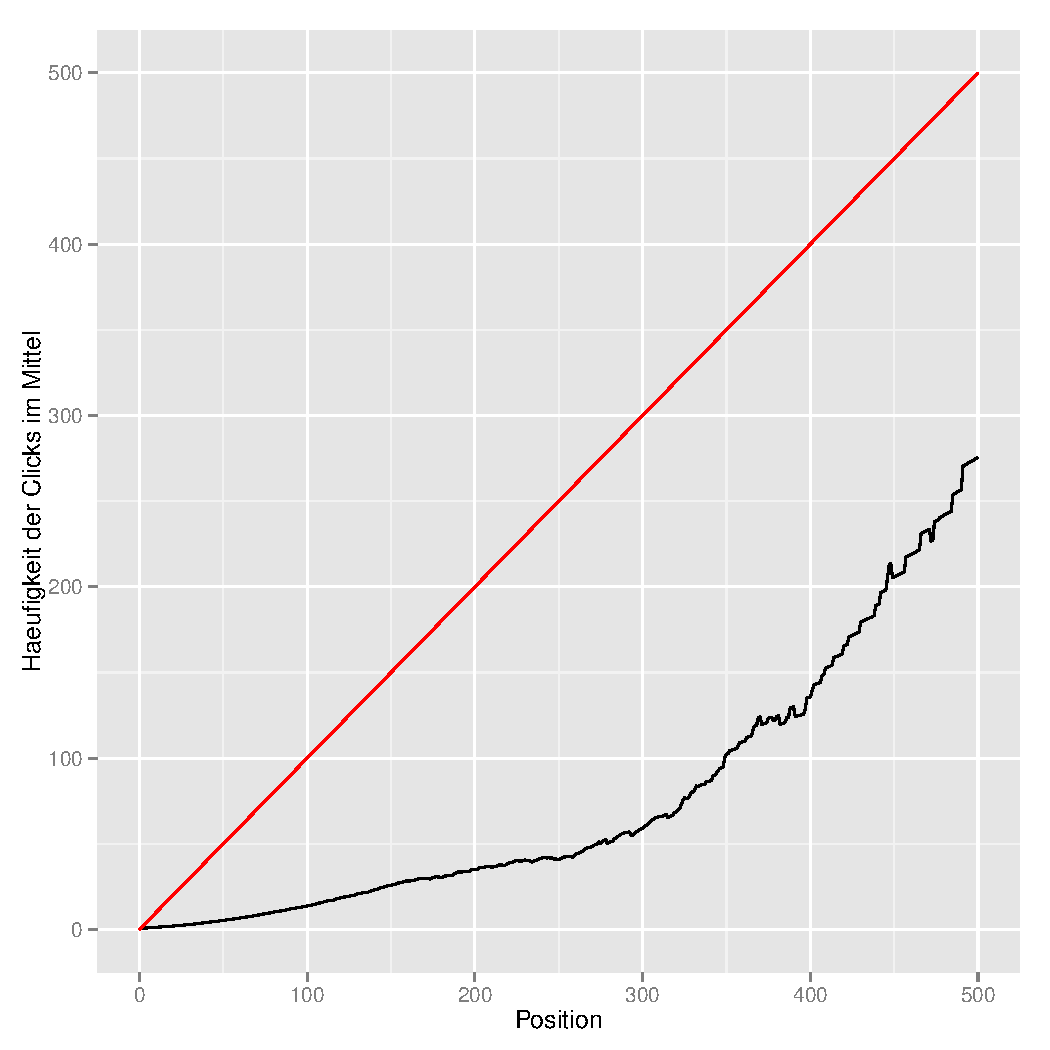
\includegraphics[scale=0.39]{clickCountSucc.pdf}
		\column{4cm}
			\begin{itemize}
				\item Anzahl der Clicks bis zur aktuellen Position
				\item Gemittelt über alle konvertierten Funnels
				\item Mehr \textit{Views} als \textit{Clicks}
			\end{itemize}
	\end{columns}
\end{frame}

%\begin{frame}\frametitle{hasClicked}
	    %\centering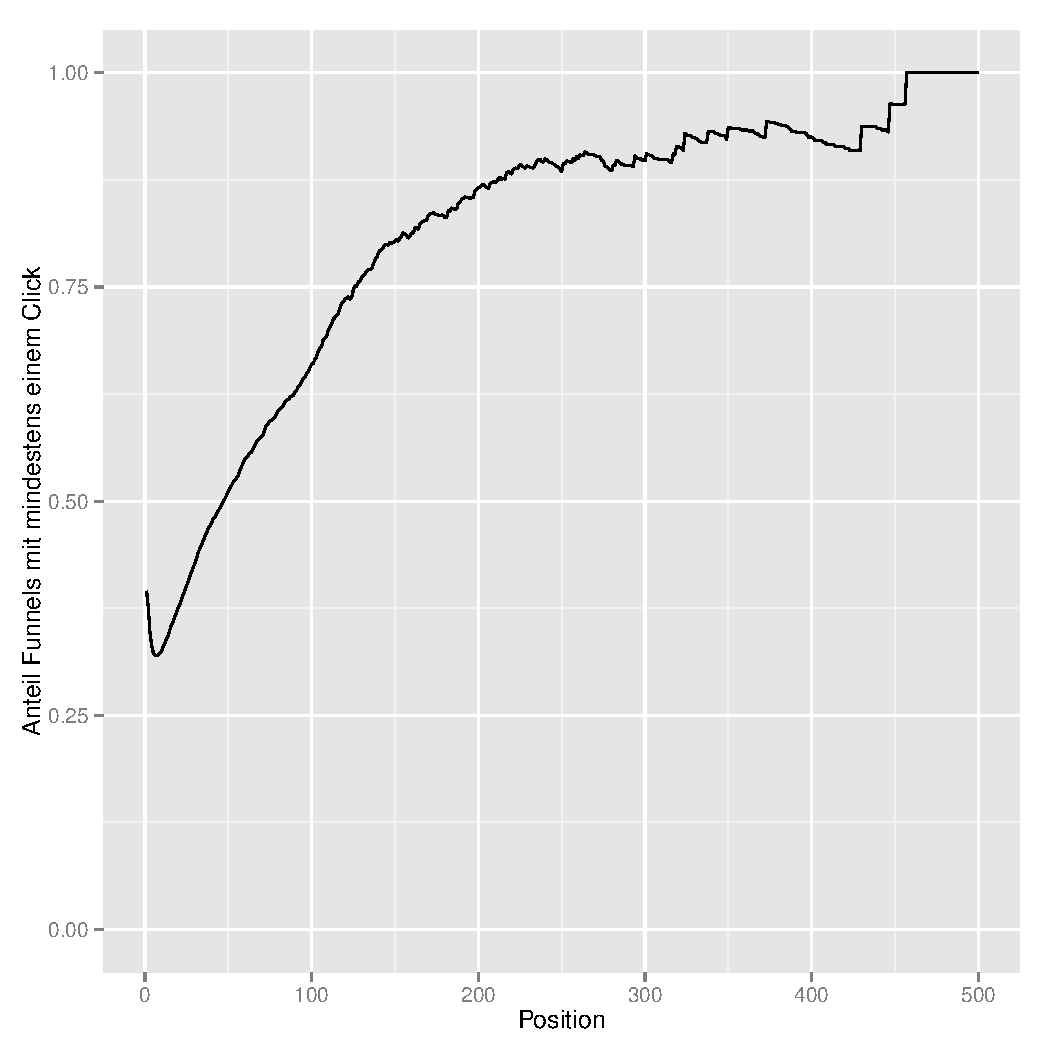
\includegraphics[scale=0.39]{hasClickedSucc.pdf}
%\end{frame}

\begin{frame}\frametitle{Beschreibung der Kampagnen}
	\begin{table}[H]
		\tiny
		\begin{center}
			\begin{tabular}{|l|p{7cm}|}
				\hline \textbf{Kampagne} & \textbf{Beschreibung}\\ \hline
				\hline Affiliate - Partnerprogramm & Partner, die Werbemittel einbinden\\
				\hline Affiliate - Rest & Partner, die Zinsvergleich bereitstellen\\ 
				\hline Direct & Direkte Eingabe von \textit{www.interhyp.de}\\ 
				\hline Display & Bannerschaltungen\\
				\hline E-Mailing & Mails an Interessenten, die schon einen Antrag o.ä. gestellt haben\\
				\hline Generic & Unbezahlter Link\\
				\hline Kooperationen - Focus & \multirow{5}{7cm}{Individuelle Zusammenarbeit mit größeren Partnern}\\
				Kooperationen - Immonet & \\
				Kooperationen - Immoscout24 & \\
				Kooperationen - Immowelt & \\
				Kooperationen - Rest & \\
				\hline Newsletter & Regelmäßige Rundschreiben\\
				\hline SEM - Brand & \multirow{3}{7cm}{Bezahlte Suchergebnisse}\\
				SEM - Remarketing & \\
				SEM - Generisch & \\
				\hline SEO & Unbezahlte Suchergebnisse\\
				\hline Social Media & \textit{facebook} und \textit{gutefrage.net}\\
				\hline
			\end{tabular} 
		\end{center}
	\end{table}
\end{frame}

\begin{frame}\frametitle{campaign}
	\begin{columns}
		\column{7cm}
			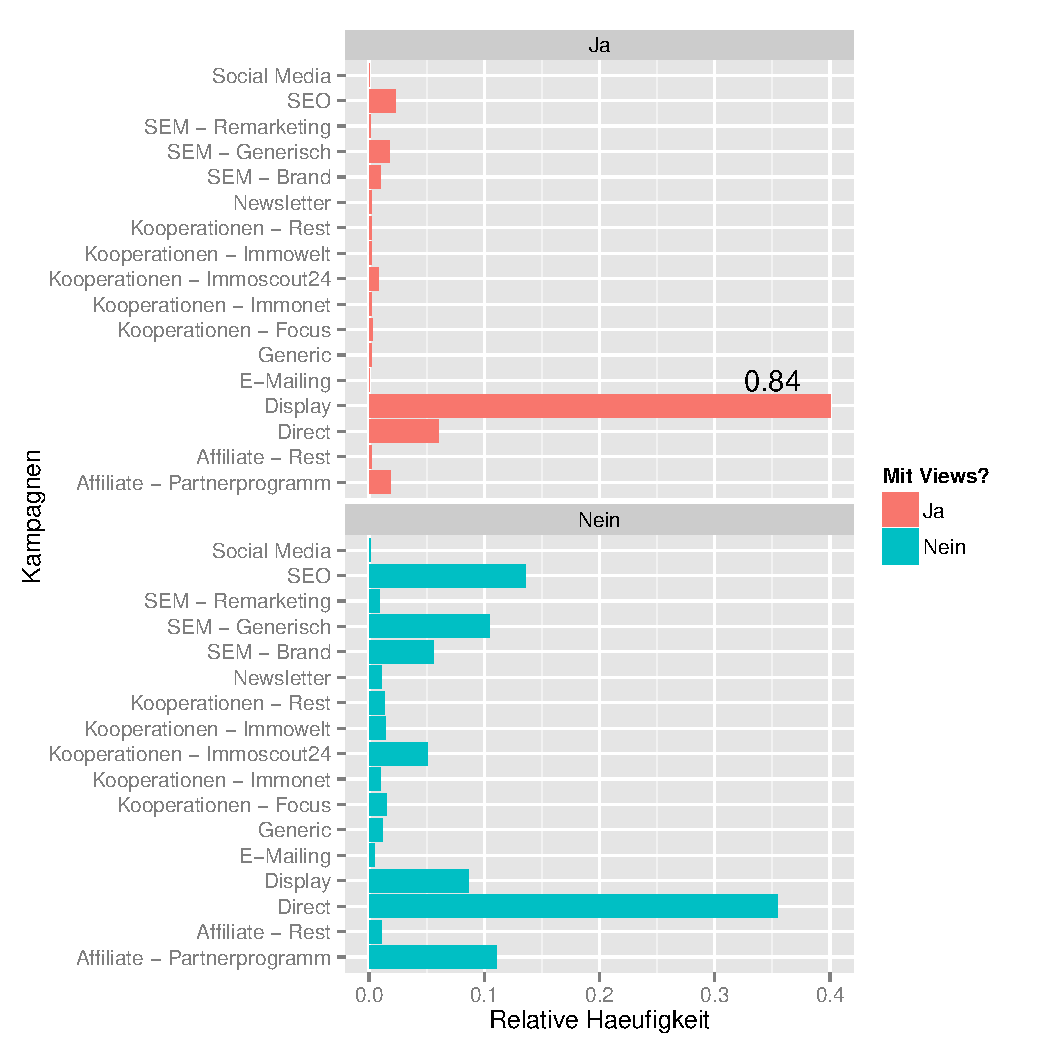
\includegraphics[scale=0.39]{campaignSucc.pdf}
		\column{4cm}
			\begin{itemize}
				\item Hauptsächlich \textit{Display} bei Berücksichtigung der \textit{Views}
				\item Ausgewogenere Verteilung wenn \textit{Views} gelöscht werden
			\end{itemize}
	\end{columns}
\end{frame}

\subsection{Vergleich von konvertierten und nicht-konvertierten Funnels}

%\begin{frame}\frametitle{weekday}
	    %\centering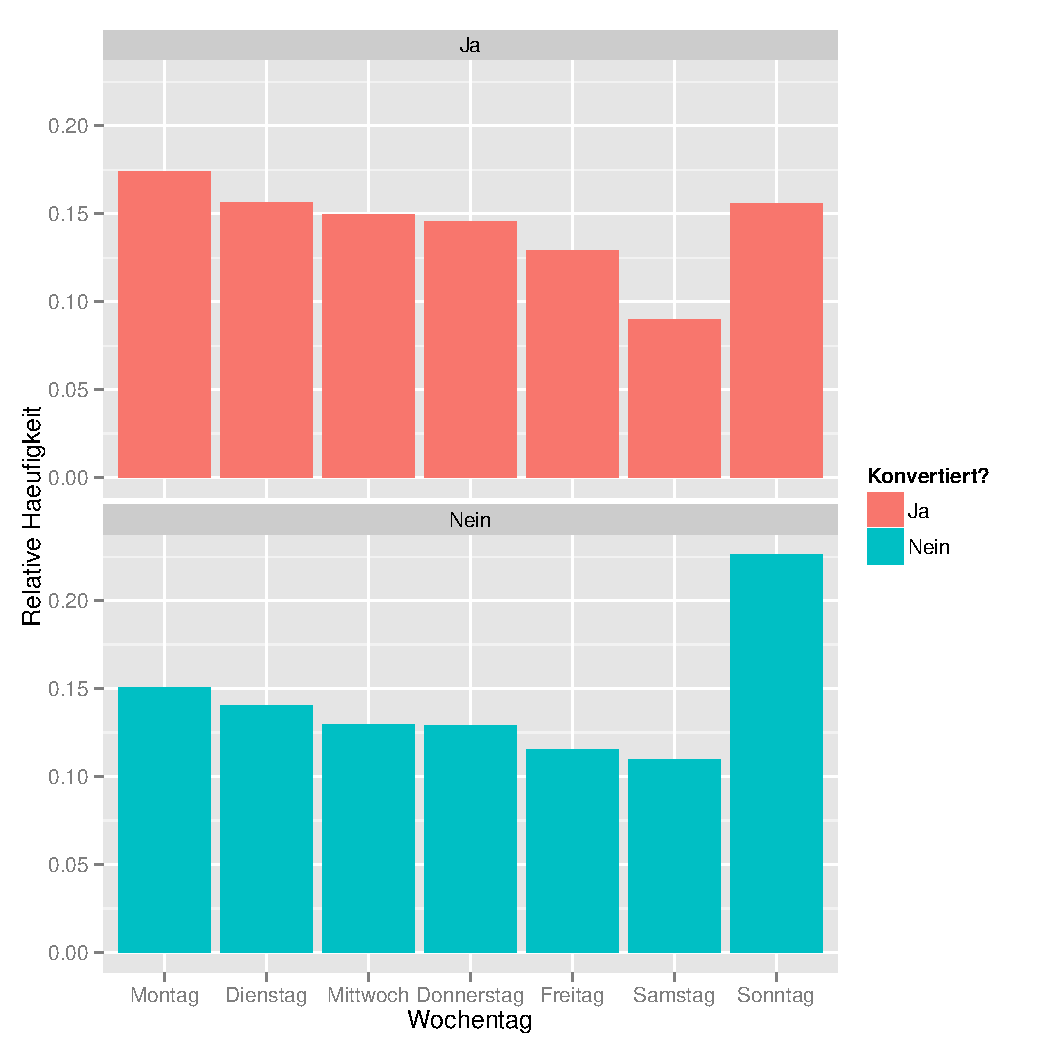
\includegraphics[scale=0.3]{weekday.pdf}
%\end{frame}

%\begin{frame}\frametitle{hour}
	    %\centering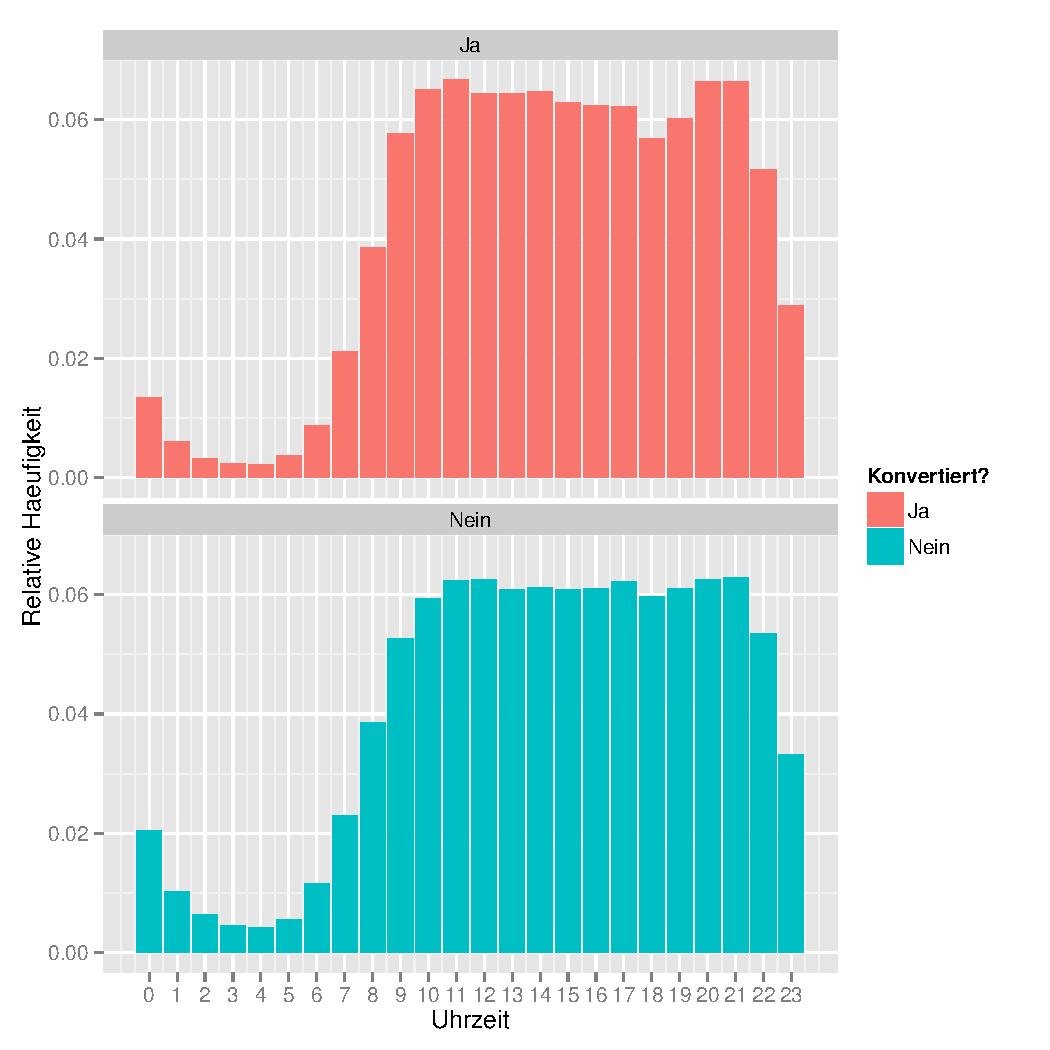
\includegraphics[scale=0.3]{hour.pdf}
%\end{frame}

\begin{frame}\frametitle{campaign}
	\begin{columns}
		\column{7cm}
			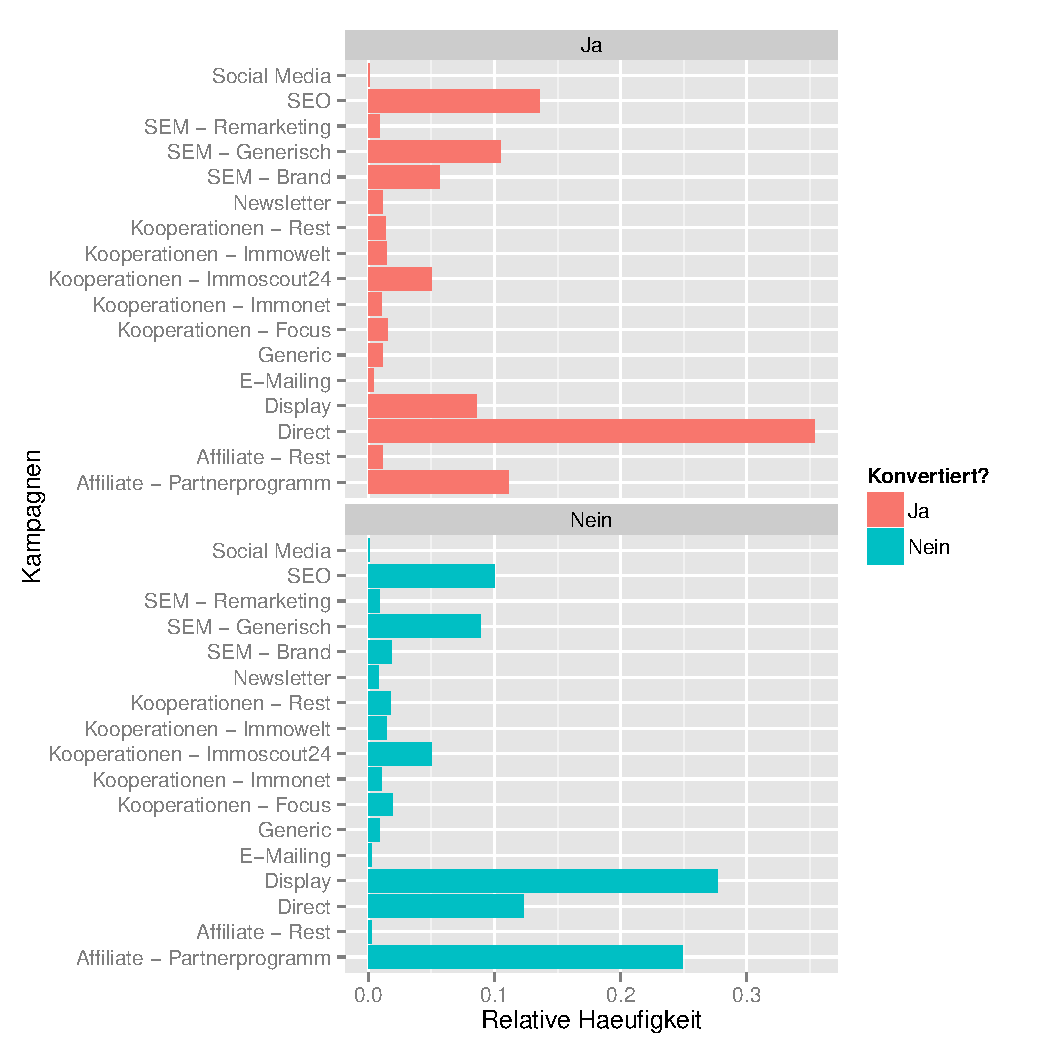
\includegraphics[scale=0.39]{campaign.pdf}
		\column{4cm}
			\begin{itemize}
				\item \textit{Direct} am häufigsten in den konvertierten Funnels
				\item \textit{Display} und \textit{Affiliate - Partnerprogramm} am häufigsten in den nicht-konvertierten Funnels
			\end{itemize}
	\end{columns}
\end{frame}

\begin{frame}\frametitle{funnelLength}
	\begin{columns}
		\column{7cm}
			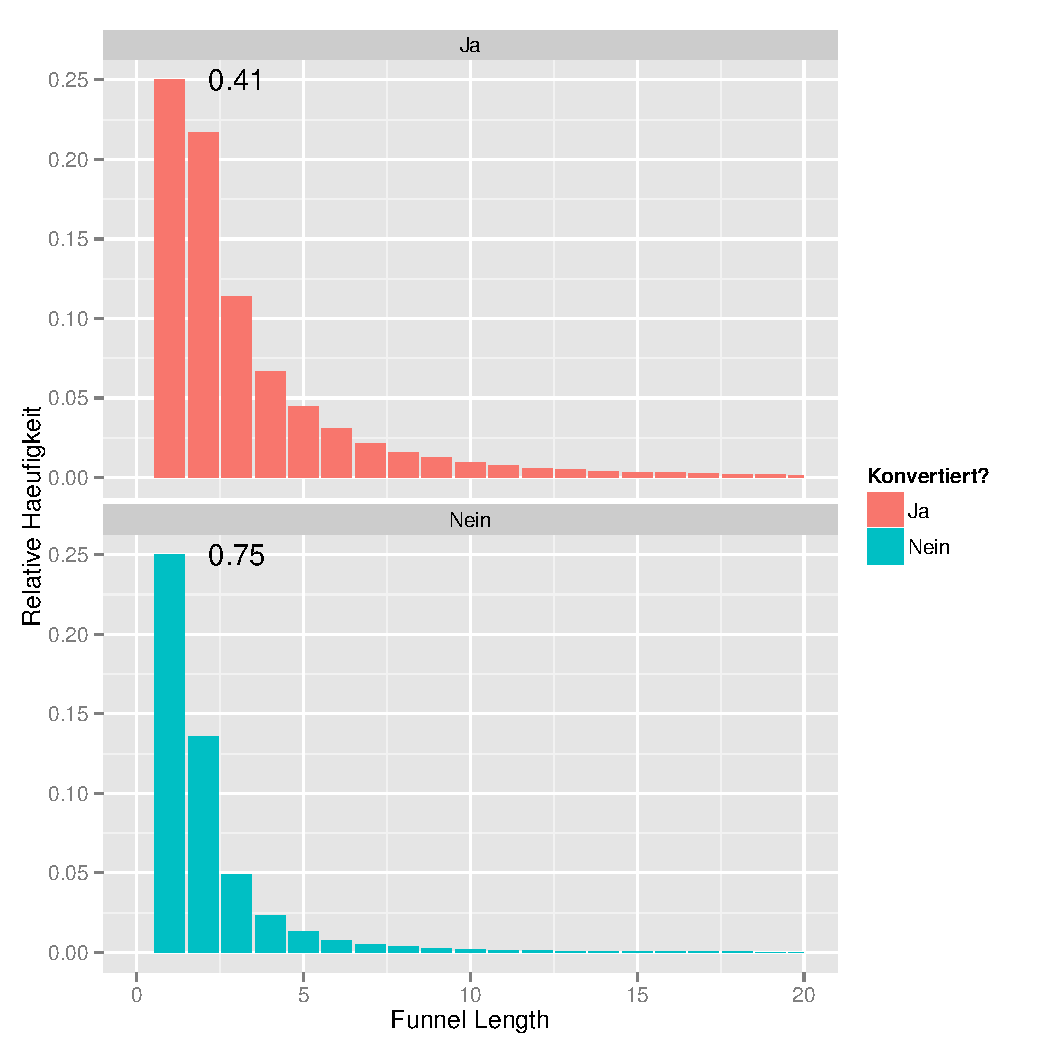
\includegraphics[scale=0.39]{funnelLength_First.pdf}
		\column{4cm}
			\begin{itemize}
				\item Anzahl Kontaktpunkte eines Funnels
				\item Kurze Funnels überwiegen deutlich
			\end{itemize}
	\end{columns}
\end{frame}

\begin{frame}\frametitle{timeSinceFirst}
	\begin{columns}
		\column{7cm}
			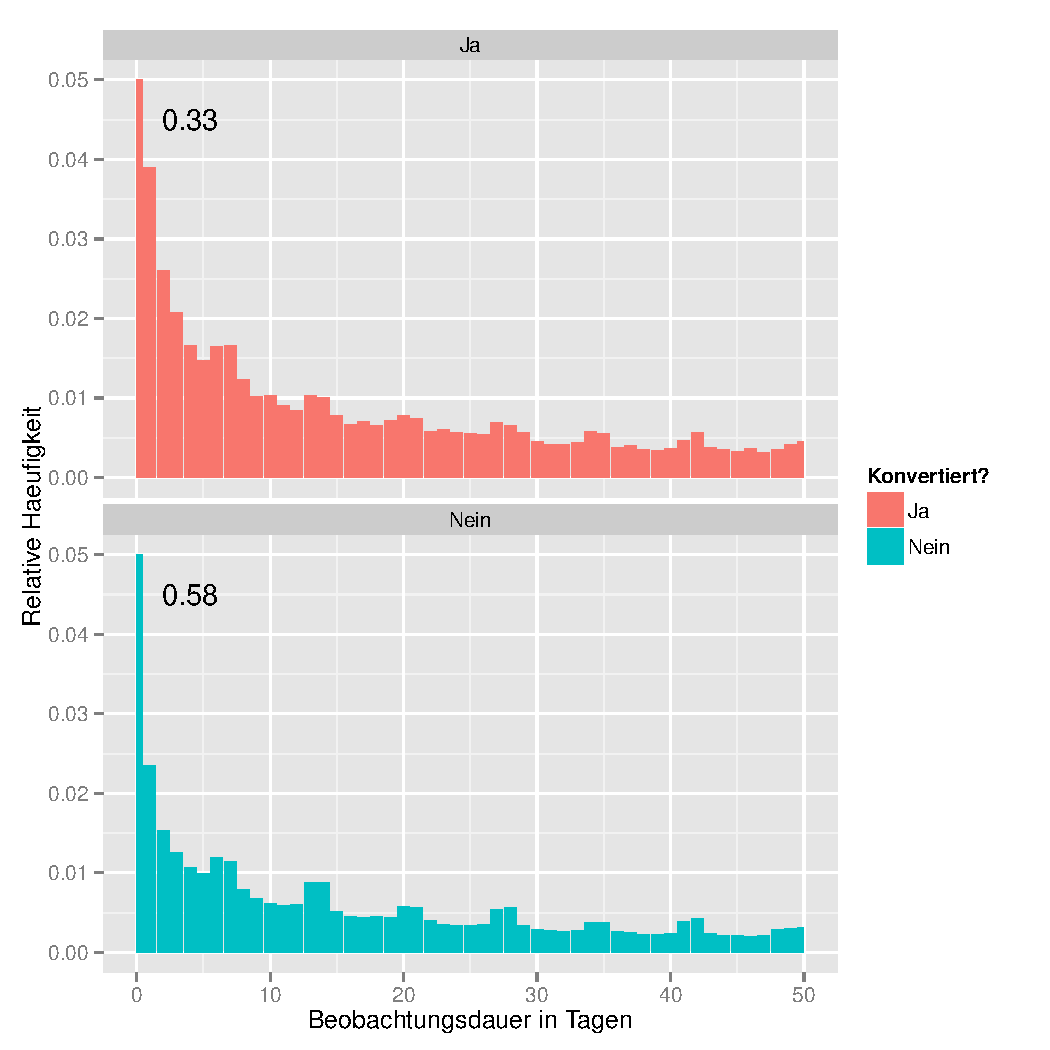
\includegraphics[scale=0.39]{timeSinceFirst_Last.pdf}
		\column{4cm}
			\begin{itemize}
				\item Verstrichene Zeit seit dem ersten Kontaktpunkt
				\item In der Abbildung wird nur der letzte Kontaktpunkt berücksichtigt
				\item Funnels mit Länge $1$ unberücksichtigt
				\item \textit{timeSinceLast}: Verstrichene Zeit seit dem vorherigen Kontaktpunkt
			\end{itemize}
	\end{columns}
\end{frame}

%\begin{frame}\frametitle{timeSinceLast}
	%\begin{columns}
		%\column{7cm}
			%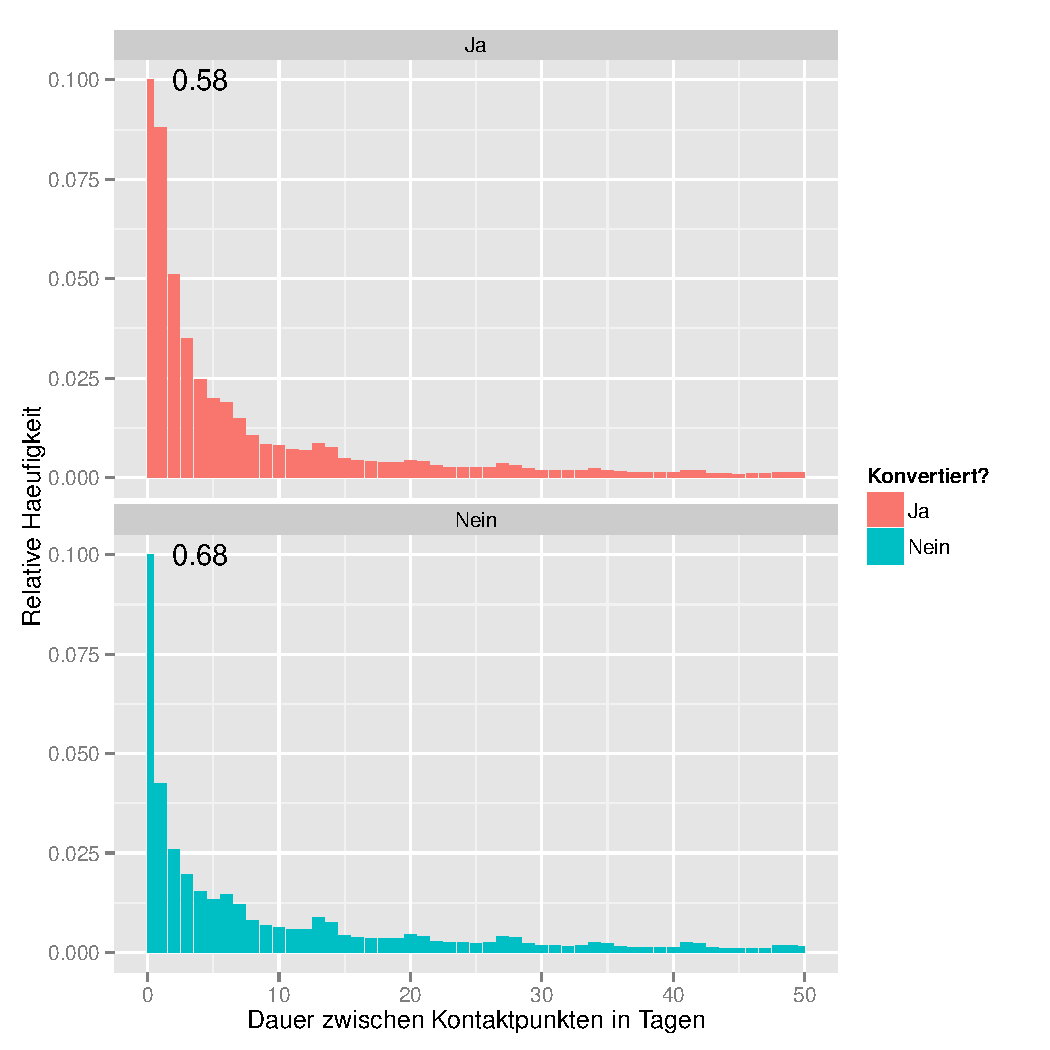
\includegraphics[scale=0.39]{timeSinceLast.pdf}
		%\column{4cm}
			%\begin{itemize}
				%\item 
			%\end{itemize}
	%\end{columns}
%\end{frame}

\begin{frame}\frametitle{freq}
	\begin{columns}
		\column{7cm}
			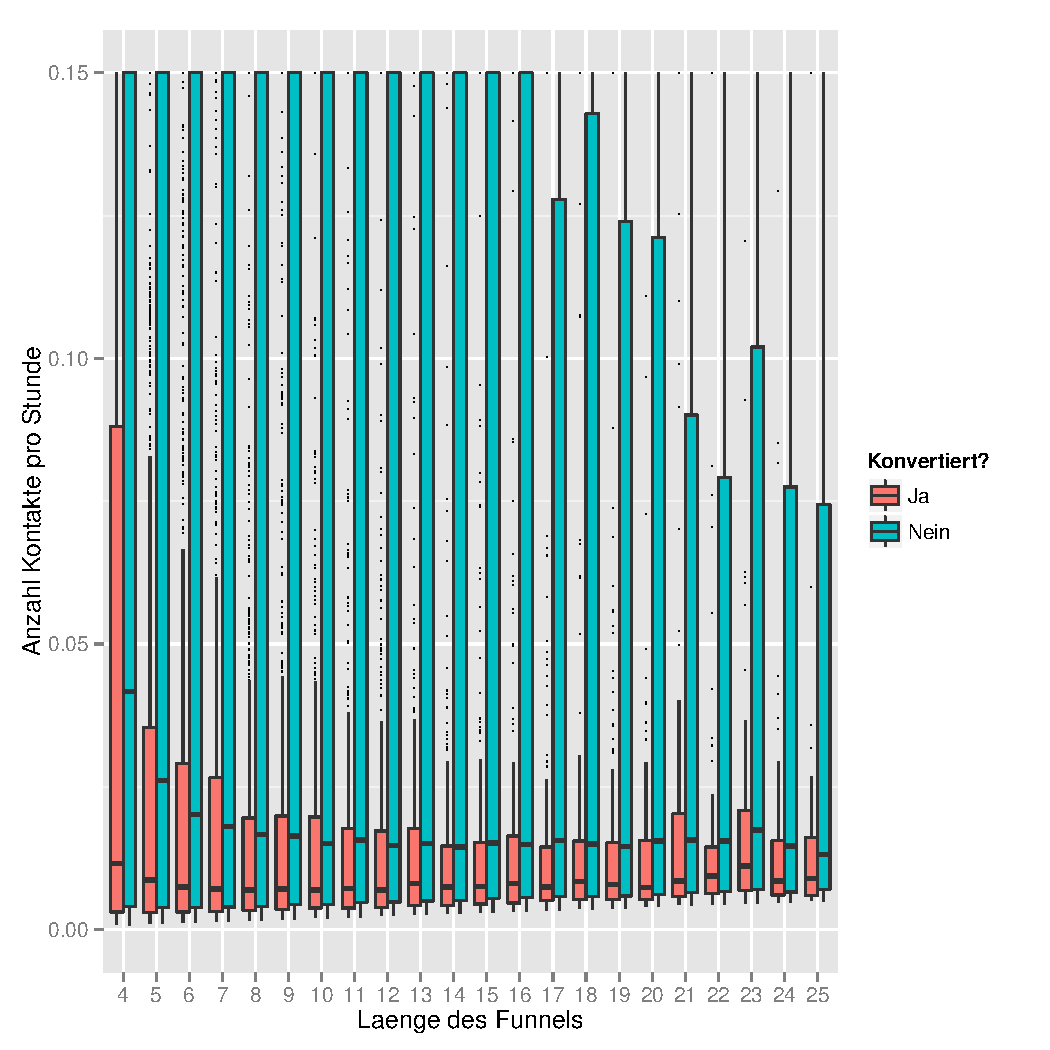
\includegraphics[scale=0.39]{freq.pdf}
		\column{4cm}
			\begin{itemize}
				\item \textit{funnelLength} dividiert durch Gesamt-Beobachtungsdauer in Stunden
				\item Frequenzen in nicht-konvertierten Funnels höher
			\end{itemize}
	\end{columns}
\end{frame}
